\section{Introduction}~\label{intro}

Recent advances in robotic systems have improved autonomy in perception, manipulation, and planning, but robots still face perception errors~\cite{kaipa2016addressing}, execution failures~\cite{kaelbling1998planning}, and unexpected environmental changes~\cite{kurniawati2016online}. In such environments, human operators can help recover from these failures~\cite{dragan2013legibility, goodrich2008human}, but continuous monitoring is impractical in long-horizon tasks because it increases workload and fatigue~\cite{chen2014human}. Robots should therefore recognize uncertain situations during execution and request assistance only when needed~\cite{sadigh2017active, leusmann2023understanding}. This raises two fundamental questions: \textit{when should a robot ask}, and \textit{what information should it request?}


Recent uncertainty-aware systems selectively request human feedback during task execution~\cite{ren2023robots, liang2024introspective, mullen2025lbap}. These approaches can reduce unnecessary intervention and improve decision making under uncertainty. However, uncertainty estimation, query generation, and planning are often treated separately, making it difficult to reason about how feedback will affect downstream execution. The link between when to ask, what to ask, and how the answer should change planning remains insufficiently explored.


To address this challenge, we present a knowledge-based decision-making framework that integrates uncertainty estimation, query selection, and symbolic planning. We formulate decision making as a partially observable Markov decision process (POMDP)~\cite{kaelbling1998planning} and represent task knowledge using a STRIPS-style symbolic model~\cite{davis1993knowledge,fikes1971strips}. During execution, the robot tracks multiple possible world hypotheses and refines them using incoming observations. If the remaining hypotheses cannot be reliably distinguished, the robot requests human feedback to resolve the ambiguity. Otherwise, it proceeds with autonomous planning and execution.


% \begin{figure}[t]
% \captionsetup{skip=0pt}
% \centering
% 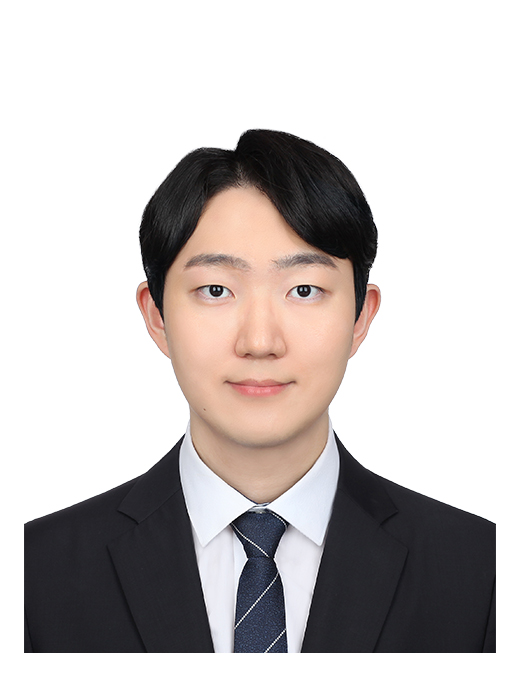
\includegraphics[width=0.5\linewidth]{figures/intro_and_method/fig_intro.jpg}
% \caption{Overview of the proposed framework. A centralized knowledge base connects sensing, planning, feedback management, and user interaction. The robot maintains uncertainty over symbolic world hypotheses and uses this uncertainty to decide whether to continue autonomous execution or request state-level feedback.}
% \label{fig:intro}
% \end{figure}


To demonstrate real-world feasibility, the framework is implemented in a robotic system architecture with sensing, planning, feedback management, and user interface modules connected through a centralized knowledge base. Observations and user feedback continuously narrow the set of plausible world hypotheses represented in the planner. This allows the robot to continue autonomous execution and request feedback only if additional information is useful.


We validate the approach in two representative robotic domains (tomato harvesting and waste sorting) through system experiments and a Wizard-of-Oz user study. The system evaluation examines query timing, query content, comparisons with baseline policies, and scalability under increasing task complexity. The user study evaluates task performance, interaction time, workload, and situation awareness to assess the impact of different query strategies on human--robot interaction. Overall, the results show that state-level querying can resolve task-relevant ambiguity with fewer interactions than existing querying policies while maintaining comparable or higher task success.
The main contributions of this work are as follows:

\begin{itemize}

\item We propose an uncertainty-aware feedback trigger method that decides \textit{when} the robot should ask for help.

\item We introduce an information-driven query selection approach to decide \textit{what} the robot should ask to reduce ambiguity among competing world hypotheses.

\item We integrate uncertainty estimation, feedback requests, and symbolic planning into a single execution loop.

\item We demonstrate that the proposed framework can improve task performance while reducing unnecessary human feedback through system experiments in two representative robotic domains.
\end{itemize}
